%-------------------------------------
\documentclass[12pt]{article}
\usepackage{amsmath}
\usepackage{amssymb}
\usepackage{epsfig}
\usepackage{xspace}
\usepackage{float} 
\usepackage{multirow}
\usepackage{pgf}
\usepackage{soul}
%\usepackage{url}
\usepackage[top=2cm, bottom=2cm, left=2cm, right=2cm]{geometry}
\usepackage{minitoc}
\usepackage{bbold}
\usepackage[nottoc,numbib]{tocbibind}

%--------------------------
\usepackage{hyperref}

%--------------------------
\usepackage{enumitem}
\setlist{noitemsep}
%\setlength\parindent{0pt}
\usepackage{algorithm}

\renewcommand*\ttdefault{txtt}


% Algorithm commands
\newcommand{\inArray}[1]{\begin{array}{l}#1\end{array}}
\newcommand{\algoNew}[1]{
  $
  \begin{array}{l}
    #1
  \end{array}
  $
}
\newcommand{\algoLine}[1]{\text{#1}\\}
\newcommand{\algoSection}[2]{\text{\textbf{#1}}\\
  \;\;\;\;\begin{array}{l}
      #2
  \end{array}\\
}
\newcommand{\algoOpen}[2]{
  \algoLine{#1}
  \left|\;
    \begin{array}{l}
      #2
    \end{array}
  \right.  \\
}
\newcommand{\algoFont}[1]{\textbf{\tt #1}}
\newcommand{\algoAfterBlockVSpace}{\vspace{0.08cm}} % Default: \vspace{0.08cm}
\newcommand{\algoBlockVerticalLine}{\hspace{0.3cm}} % Default:\hspace{0.3cm}
\newcommand{\algoBlockVerticalSpace}{\hspace{-0.1cm}} % Default: \hspace{-0.1cm}

\newcommand{\algoBox}[3]{
  \begin{array}{| l @{} l}
      \cline{1-1}
      \multicolumn{2}{|l}{\algoBlockVerticalSpace\text{#1}  }\\
      \algoBlockVerticalLine & \inArray{#2} \\
      \multicolumn{2}{|l}{\algoBlockVerticalSpace\text{#3} }\\
      \cline{1-1}
  \end{array}\algoAfterBlockVSpace\\
}

\newcommand{\algoBoxIfElse}[5]{
  \begin{array}{| l @{} l}
      \cline{1-1}
      \multicolumn{2}{|l}{\algoBlockVerticalSpace\text{#1}  }\\
      \algoBlockVerticalLine & \inArray{#2} \\
      \multicolumn{2}{|l}{\algoBlockVerticalSpace\text{#3} }\\
      \algoBlockVerticalLine & \inArray{#4} \\
      \multicolumn{2}{|l}{\algoBlockVerticalSpace\text{#5}  }\\
      \cline{1-1}
  \end{array}\algoAfterBlockVSpace\\
}
\newcommand{\algoEnd}{\algoLine{end}}



\definecolor{Red}{rgb}{1,0,0}
\definecolor{Green}{rgb}{0,0.6,0.4}
\definecolor{Blue}{rgb}{0,0,1}
\definecolor{Gray}{rgb}{0.2,0.2,0.2}




% A crossed-out Rightarrow
%\newcommand{\doesNotImply}{
%  \text{\mbox{
%    $\not{\!\!\Rightarrow}$
%  }}
%}



% Various notations
\def\R{{\mathbb{R}}}
\def\N{{\mathbb{N}}}
\def\Z{{\mathbb{Z}}}
\def\P{{\mathbb{P}}}
\def\E{{\mathbb{E}}}
\def\L{{\mathcal{L}}}

\newcommand{\y}{\mathbf{y}}
\renewcommand{\c}{\mathbf{c}}
\newcommand{\I}{\mathbf{I}}
\newcommand{\A}{\mathbf{A}}
\newcommand{\x}{\mathbf{x}}
\newcommand{\z}{\mathbf{z}}
\newcommand{\w}{\mathbf{w}}
\newcommand{\W}{\mathbf{W}}
\renewcommand{\H}{\mathbf{H}}
\newcommand{\h}{\mathbf{h}}
\renewcommand{\b}{\mathbf{b}}
\renewcommand{\u}{\mathbf{u}}
\newcommand{\Yh}{\mathbf{\hat{Y}}}
\newcommand{\under}{\texttt{\char`\\}}
\newcommand{\dynatree}{{\sf dynaTree}\xspace}
\newcommand{\tgp}{{\sf tgp}\xspace}
\newcommand{\sgtelib}{{\sf sgtelib}\xspace}
\newcommand{\nomad}{{\sf Nomad}\xspace}
\newcommand{\mads}{{MADS}\xspace}

\newcommand{\fh}{\hat{f}}
\newcommand{\ch}{\hat{c}}
\newcommand{\sh}{\hat{\sigma}}
\newcommand{\yh}{\hat{y}}
\newcommand{\ycv}{\hat{\y}^{cv}}


\newcommand{\eh}{\hat{\varepsilon}}
\newcommand{\sbar}{\overline{\sigma}}
\newcommand{\sbars}{\overline{\sigma}_u}
\newcommand{\sbary}{\overline{\sigma}_d}
\newcommand{\ybar}{\overline{y}}
\newcommand{\kmax}{{k_{max}}}
\newcommand{\fmin}{f_{min}}

\renewcommand{\chi}{\mathcal{X}}
\newcommand{\fm}{f_{min}}
\newcommand{\X}{\mathbf{X}}
\newcommand{\var}{\mathbb{V}\text{ar}}
\newcommand{\gaussian}{\mathcal{G}}

\newcommand{\FS}{F\!\sigma}
\newcommand{\FSP}{F\!\sigma\!P}
\newcommand{\EI}{E\!I}
\newcommand{\EFI}{E\!F\!I}
\newcommand{\EIS}{E\!I\!\sigma}
\newcommand{\EFIS}{E\!F\!I\!\sigma}
\newcommand{\EFIC}{E\!F\!I\!C}
\newcommand{\EFIM}{E\!F\!I\!\mu}
\newcommand{\PI}{P\!I}
\newcommand{\PFI}{P\!F\!I}
\newcommand{\FU}{\mu}

\newcommand{\ind}{\mathbb{1}}

\newcommand{\metric}{\mathcal{E}}
\mathchardef\mhyphen="2D
\newcommand{\Mrmse}{\metric_{RMSE}}
\newcommand{\Mpress}{\metric_{RMSECV}}
\newcommand{\Mlinv  }{\metric_{LINV}}

\newcommand{\instance}{\rho}
\newcommand{\instanceMax}{\instance_{\max}}



%\newcommand{\xp}{{\x^{proj}}}
\newcommand{\xP}{\x^P_t}
\newcommand{\xS}{\x^S_t}
\newcommand{\xBest}{\x^*_t}
\newcommand{\mesh}{\mathcal{M}}
%\renewcommand{\S}{\mathbf{S}}
%\newcommand{\xtry}{\x^{try}}

\newcommand{\proj}{\text{proj}}


\newcounter{modelIndex}
\addtocounter{modelIndex}{1}
\newcommand{\modelIndex}{
  \arabic{modelIndex}\addtocounter{modelIndex}{1}
}



% Other commands
\newcommand{\figureWidth}{0.95\linewidth}

\renewcommand{\quote}[1]{``#1''}
\newcommand{\figWidth}{12cm}

\newcommand{\mynote}[1]{
%\colorbox{blue!30}{
%\begin{minipage}[c]{8cm}
  \textbf{\underline{Note}:~#1}
%\end{minipage}
%}
}
%\textcolor{red}{\textbf{\underline{Note}:~#1}}
\renewcommand{\mynote}[1]{\textcolor{red}{\textbf{[EDIT]}~#1}}



\newcommand{\seb}{}%\color{Green}}
\newcommand{\mk}{}%\color{Red}}

\newcommand{\ignore}[1]{}


\renewcommand{\t}{^\top}
\newcommand{\shortMinus}{\mathord{-}}
%\renewcommand{\shortMinus}{\text{-}}
\newcommand{\noti}{^{(\text{-}i)}}
\newcommand{\notj}{^{(\text{-}j)}}



%\usepackage{setspace}
%\doublespacing

%--------------------------
\title{Engage Project Technical Report:\\
Surrogate Models for Maximizing Net Present
Value of Renewable Energy Sources
}
\author{Bastien Talgorn and Michael Kokkolaras\\
Department of Mechanical Engineering\\
McGill University}
%\date{}
%--------------------------



%--------------------------------------         
\begin{document}
%--------------------------------------


\maketitle
\setlength{\parindent}{0pt}

\tableofcontents




%==========================================%
%==========================================%
\section{Overview of surrogate modeling techniques}
\label{sec:models}
%==========================================%
%==========================================%


From a set of observations $[\X,\y]$, 
  with $\X=\{\x_1,....,\x_p\} \subset \R^n$ and 
  $\y = y(\X)$ (i.e.: $\y_i = y(\x_i)$) 
  where $y:\R^n\rightarrow \R$ is either the objective function $f$ 
  or one of the constraint functions $\{c_j\}_{j\in J}$, 
  it is possible to build a surrogate model $\yh$ 
  which can be used to predict the value of $y(\x)$ for $\x\notin\X$.
In this section, we describe three types of surrogate models and how to use them to build an ensemble of surrogates:
Polynomial Response Surfaces (PRS)
\cite{AcarOptimizedWeight2009,MullerMixtureSurrogate2011,QueipoSbao2005},
Kernel Smoothing (KS)
\cite{AcarOptimizedWeight2009,hastie01statisticallearning}, 
and Radial Basis Functions (RBF)
\cite{buhmann2003radial,AcarOptimizedWeight2009,VianaEgoMusu2013,MullerMixtureSurrogate2011,QueipoSbao2005}.    


%We will see in Section \ref{sec:ensemble} that  in order 
To quantify the quality of a surrogate model, 
  it is useful to compute,
for each training point $\x_i\in \X$, 
  the value that $\yh(\x_i)$ would have taken if the model $\yh$ 
  had been built without the observation $[\x_i,y(\x_i)]$. 
Thus, we define $\yh\noti$ the surrogate model built by leaving out the observation $[\x_i,y(\x_i)]$ for $\x_i \in \X$. We also define the cross-validation vector $\ycv$ such that $\yh^{cv}_i = \yh\noti(\x_i)$.

%As PRS and RBF models both fall in the category of linear models (not to be mistaken with linear regression), Section \ref{sec:linear} presents an overview for these types of model.

%-------------------------------------------%
\subsection{Linear models}
\label{sec:linear}
%-------------------------------------------%
\renewcommand{\a}{\boldsymbol{\alpha}}


A model $\yh$ is said to be linear if it can be expressed as a linear combination of basis functions \cite{mardia1979multivariate,STIGLER1974431,Gergonne1974439,orr1996introduction}:
\begin{equation}
  \yh(\x) = \sum_{j=1}^q \alpha_j h_j(\x),
\end{equation}
where $h_j(x):\R^n\rightarrow\R$ is a (possibly non-linear) basis function. 
The coefficients $\a = [\alpha_1,...,\alpha_q]\t$ are computed to minimize the regularized quadratic error of the model
\begin{displaymath}
  \sum_{\x\in\X} (y(\x)-\yh(\x))^2 + r_{ridge} \|\a\|^2_2,
\end{displaymath}
where $r_{ridge} \ge 0$ is a regularization (or ridge \cite{orr1996introduction}) parameter. This parameter ensures that the linear system is invertible, even if there are more basis functions than training points or if the training points are aligned. 
In the case where the number of training points does not exceed the number of basis functions (
  $p\le q$), the model is constructed only if the ridge coefficient is not null. 
Otherwise, the model will be built only when more training points become available. 

For such models, the \emph{design matrix} $\H$ can be built from the training points $\X = \{\x_1,\x_2,...,\x_p\}$:
\begin{equation}
  \H  
  =\left[\begin{array}{c c c}
    h_1(\x_1) & ... & h_q(\x_1) \\
      \vdots  &     & \vdots  \\
    h_1(\x_p) & ... & h_q(\x_p) \\
  \end{array}\right].
  \label{eq:design-matrix}
\end{equation}
Note that the matrix $\H$ is independent from the output $y(\X)$. To solve this kind of problem, we consider only the cases where the number of training points is larger than the number of basis functions (i.e. the number of unknown coefficients) or where the ridge coefficient is not null. In these two cases, the use of ordinary least squares (OLS) is required. The coefficients $\a$ are then the solution of the invertible problem:
\begin{equation}
  \underset{\A}{\underbrace{(\H\t \H+r_{ridge} \I_q)}}\a = \H\t\y. 
\end{equation}
It follows that
\begin{equation}
  \a  = \A^{-1} \H\t \y.
\end{equation}



An interesting property of this kind of model is that the cross-validation vector can easily be computed by
\begin{equation}
  \ycv  = \y- diag({\mathbf P})^{-1} {\mathbf P} \y,
\end{equation}
where ${\mathbf P}$ is the \emph{projection} matrix \cite{orr1996introduction} such that ${\mathbf P} = \I_p - \H \A^{-1} \H\t$ and $diag({\mathbf P})$ is the diagonal matrix such that $diag({\mathbf P})_{ii} = P_{ii}$.
Once the design matrices $\H$ and $\A$ are built and $\A^{-1}$ has been computed for one given function $y$, it is really inexpensive to compute the coefficients $\a$ for other functions $\y$
 (for example, each output of the blackbox) and to compute the cross-validation values.

%-------------------------------------------%
\subsection{Polynomial Response Surfaces}
%-------------------------------------------%
\label{sec:PRS}
Polynomial response surfaces are linear models for which the basis function are polynomials. For a PRS of degree $d$, the set of basis functions $\{h_j\}_{j=1,...,q}$ is a basis of the polynomial vector space of degree $d$ in $\R^n$. 

%-------------------------------------------%
\subsection{Radial Basis Functions}
\label{sec:RBF}
%-------------------------------------------%

RBF models rely on basis functions which follow the form $h_j(\x) = \phi(d(\x_j,\x))$, where $d$ is a distance function (in our case, the Euclidean distance) and $\phi:\R_{\ge 0}\rightarrow \R $ is a kernel function. \mynote{Note that kernel functions are general mathematical concepts that are also used in other modeling techniques like Kernel Smoothing or Kriging.} In most studies on RBFs
\cite{buhmann2003radial,orr1996introduction,
GoelErrorCriteria2009,AcarOptimizedWeight2009,VianaEgoMusu2013}, the coefficient of the RBF models are obtained by solving the square linear system

\begin{equation}
  \left[ \begin{array}{c c}
    \H^{RBF} & \H^{PRS} \\
    (\H^{PRS})\t & 0 \\
    \end{array}
  \right] \a = \left[ \begin{array}{c}
    \y \\
    0 \\
    \end{array}
  \right],
  \label{eq:rbf-std}
\end{equation}
where $\H^{RBF}$ is a symmetric matrix such that $H_{ij} = \phi(d(\x_i,\x_j))$ and $\H^{PRS}$ is the design matrix of a PRS of degree 1, as described in the previous section. 

The main flaw of this method is that the computational cost of building an RBF model can become prohibitive for a large number of training points. 
\mynote{We propose a novel class of RBF models, denoted RBFI where the \quote{I} stands for \quote{Incomplete basis}. This class of models relies on the reduction of the} number of basis functions by carefully selecting a subset of the training points $S(\X) = \{\x_i^s \}_{i=1,...,q^{RBF}} \subset \X$. 
This subset contains $q^{RBF} < p$ training points of $\X$ on which will be centered the radial basis functions. 
The matrix $\H^{RBF}$ is then defined in $\R^{p\times q^{RBF}}$ such that $H^{RBF}_{ij} = \phi(d(\x_i,\x_j^s)) \; \forall i=1,...,p \; \forall j=1,...,q^{RBF}$. 
The design matrix is defined as $\H = [\H^{RBF} \; \H^{PRS}]$, where $\H^{PRS}$ is the PRS design matrix of size $p \times q^{PRS}$. 
Consequently, the total number of basis function in this model is $q=q^{RBF}+q^{PRS}$. We chose $q^{RBF} = \min\{p/2 , 10n\} $. 
 That means that only $q^{RBF}$ radial basis function are selected but they are merged with $q^{PRS}$ PRS basis functions. The PRS used in this work is of degree 1. That means that $q^{PRS} = n+1$. As the system is overdetermined, we don't need to add orthogonality constraints like in equation \eqref{eq:rbf-std}. The coefficient $\a$ are computed with normal equations as described in Section \ref{sec:linear}. 

To build the set $S(\X)$, we use a greedy algorithm that is computationally efficient and robust in selecting $p_S$ points in the set $\X$. This novel algorithm is described in Algorithm \ref{algo:selection}. It takes as an input the training set $\X$, the incumbent solution $x^*$, and the number of selected kernels is set to $\min\{p/2,100\}$.

\newcommand{\Sin}{S_{in}}
\newcommand{\Sout}{S_{out}}
\newcommand{\pS}{p_{out}}
\newcommand{\xtarget}{\x_{0}}

\begin{algorithm}
\algoNew{
    \algoLine{Input : $\Sin$, $\xtarget$ and $\pS$}
    \algoSection{[1] Initialization}{
      \algoLine{Randomly draw  $\x_{new}$ in $\Sin \under \{\x^*\}$ }
      \algoLine{$\Sout \leftarrow \{\x_{new}\} \cup (\xtarget \cap \Sin)$ }
      \algoLine{$\lambda \leftarrow 3$ }
      \algoLine{$\lambda_{min} \leftarrow 0.01$ }
    }% End Section

    \algoSection{[2] Greedy selection}{
      \algoOpen{while card$(\Sout) < \pS$ and $\lambda>\lambda_{min}$}{
        \algoLine{Select $\x_{new} \in \underset{\x\in\Sin}{\text{argmax}} \;\; d(\x,\Sout)\shortMinus\lambda d(\x,\xtarget)$ }
        \algoOpen{if $d(\x_{new},\Sout) = 0$}{
          \algoLine{$\lambda \leftarrow 0.99\lambda$}
        }
        \algoOpen{then}{
          \algoLine{$\Sout \leftarrow \Sout \cup \{\x_{new}\}$}
        }
        \algoEnd
      }
      \algoEnd
    }% End Section
  	\algoLine{Return $\Sout$}
  }% End Algo
  \caption{Greedy selection}
  \label{algo:selection}
\end{algorithm}	



The goal of this algorithm is to select a subset $\Sout$ of $\pS$ points from the set $\Sin \in \R^n$. The set $\Sout$ must be spread as widely as possible in $\R^n$ and yet we want to favor points of $\Sin$ that are close to a target point $\xtarget$. As these two are conflicting, a trade-off parameter $\lambda$ is introduced. 
When many points that are close to $\xtarget$ have been selected, it is possible that the pressure to select more points close to $\xtarget$ will lead to selecting a point that is already selected (leading to $d(\x_{new},\Sout)=0$). In that case, the trade-off coefficient $\lambda$ is decreased. 
An example of training points selection is shown in Figure \ref{fig:kernel-selection}. 



\begin{figure}[!ht]
	\center
  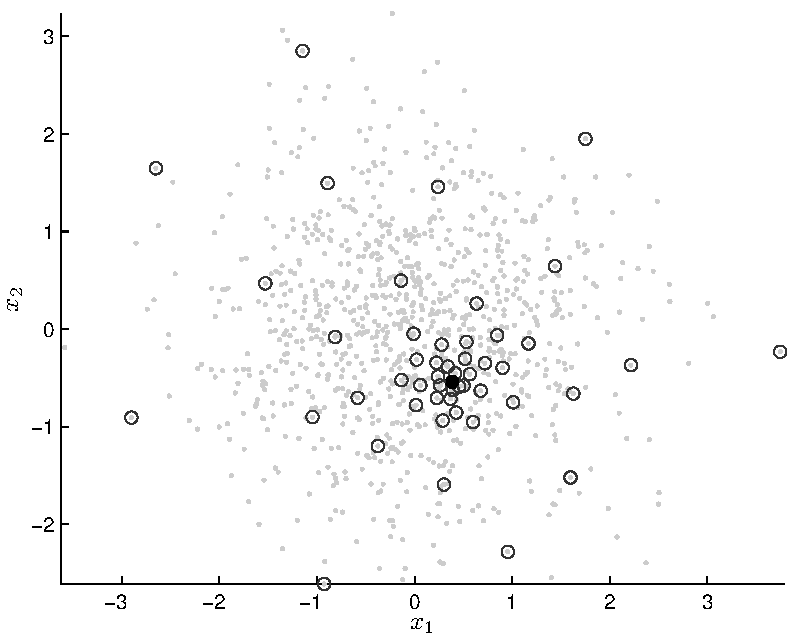
\includegraphics[width=8cm]{./includes/show_selectkernel_1.pdf}
  \caption{Selection of 100 points out of 1000 points following a Gaussian distribution in $\R^2$. The circles are the selected points.}
  \label{fig:kernel-selection}
\end{figure}






%-------------------------------------------%
\subsection{Kernel Smoothing}
\label{sec:KS}
%-------------------------------------------%

Kernel smoothing models consist of a weighted sum of the training points, where the weight decreases with the distance to the training point:
\begin{equation}
  \yh(\x) = \frac{ \sum_{i=1}^n \phi(d(\x,\x_i)) y_i }{ \sum_{i=1}^n \phi(d(\x,\x_i)) }.
\end{equation}
The advantage of KS is that the computation is immediate. It does not require a linear system inversion. One of the drawbacks is that KS rarely respects the training set, and has a tendency to ``undershoot'', that is to say that low values will be represented higher than expected and high values will be lower. However, despite their tendency to undershoot, we observe that KS models typically tend to respect the order or sign of the output. 




%-------------------------------------------%
\subsection{Ensemble of surrogates }
\label{sec:ensemble}
%-------------------------------------------%

For each (objective or constraint) function $y$ that needs to be computed, we build a set of $\kmax$ surrogate models $\yh_k$. Then, these models are aggregated into a single model using
\begin{equation}
  \yh(\x) = \sum_{k=1}^{\kmax} w_k\yh_k(\x),
\end{equation}
where $\w = [w_1,...,w_\kmax]$ is a weight vector such that $w_k\ge0$ and $\sum_{k=1}^{\kmax}w_k=1$. \mynote{To denote the difference between the ensemble of models (which is itself a model) and the models that comprise this ensemble, we will say, as a convention, that the ensemble of models is made of \quote{simple} models}. 


Many approaches have been proposed in previous studies to choose the weights $\w$ for a given set of data $[\X,y(\X)]$. Most of them \cite{VianaEnsemble2008,AcarOptimizedWeight2009,GoelEnsemble2007} rely on calculating an error metric $\metric_k$ for each surrogate $\yh_k$, then on setting $w_k \propto g(\metric_k) \ge 0$, where $g$ depends on the method chosen.
This notation is equivalent to the two-step definition: $w'_k = g(\metric_k)$, then $w_k = \frac{w'_k}{\sum_k w'_k}$.
% where $\w '$ is a set of non normalized weights such that $w_k \propto w'_k$ but $\sum w'_k \neq 1$. 


For example, \cite{GoelEnsemble2007} proposes the following weight selection methods
\begin{align}
\text{WTA1} & : \;\;\; w_k \propto \metric_{sum} - \metric_k \nonumber \\
\text{WTA2} & : \;\;\; w_k \propto \ind_{\metric_k = \metric_{min}} \nonumber \\
\text{WTA3} & : \;\;\; w_k \propto (\metric_k + \alpha \metric_{mean})^\beta, \nonumber
\end{align} 
where $\metric_{sum}$, $\metric_{min}$ and $\metric_{mean}$ are respectively the sum, minimum and mean of $\{\metric_k\}_{k=1...\kmax}$. For WTA3, the values $\alpha<1$ and $\beta<0$ must be given by the user and \cite{GoelEnsemble2007} recommends $\alpha=0.05$ and $\beta=-1$. 

The WTA2 method is tantamount to selecting the best model and, if there are several surrogates with the minimal error, sharing the weights between these models.

Another approach is to optimize the weights to minimize the error metric $\metric$ of the aggregated model. In this report, the first method used in choosing the vector $\w$ is to minimize
\begin{displaymath}
\frac{RMSECV(\w)}{1-\var(\w)},
\end{displaymath}
where RMSECV (Root mean Square Error with Cross-Validation, also called PRESS (Predicted REsidual Sum of Squares)) \cite{Allen1974,Tarpey2000} is the quadratic cross-validation error
\begin{equation}
  RMSECV(\w) = \sqrt{ \frac{1}{p} \sum_{i=1}^p \left( y(\x_i)-\sum_{k=1}^\kmax w_k\yh_k\noti(\x_i) \right)^2 },
\end{equation}
where $\yh\noti_k(\x_i)$ is the cross-validation value of the simple model $\yh_k$ in $\x_i$ and 
\begin{equation}
  \var(\w) = \frac{ \kmax\Big(\sum_{k=1}^{\kmax} w_k^2\Big) -1}{\kmax-1}
\end{equation}
is used to favor the use of several models. The second method consists of minimizing
\begin{displaymath}
\frac{1}{\mathcal{L}(\w)(1-\var(\w))},
\end{displaymath}
where $\mathcal{L}$ is the likelihood of the model, defined as


\begin{align}
  \L &= \prod_{\x\in\X} \P[y(\x) | \yh(\x),\sh^2(\x)] \nonumber \\
     &= \prod_{\x\in\X} \frac{1}{\sqrt{2\pi}\sh(\x)}
            \exp \left(
              \frac{(y(\x)-\yh(\x))^2}{\sh^2(\x)}
            \right).
\end{align}
Note that is is generally more practical and numerically-stable to compute
\begin{align}
  \log{\L} \propto \sum_{\x\in\X} -\log(\sh(\x)) + 
              \frac{(y(\x)-\yh(\x))^2}{\sh^2(\x)} \nonumber
\end{align}


The models used in the ensemble of surrogates are listed in Table \ref{tab:list-models}.


  \setcounter{modelIndex}{1}
  \begin{table}[!h]
    \caption{List of simple surrogate models}
    \label{tab:list-models}
    \center
    \begin{tabular}{| c | c | c | c |}
      \hline
      \#           & \begin{tabular}{c}Model\\type\end{tabular}  & Param. 1 & Param. 2 \\
      \hline
      % PRS ==========================
      \begin{tabular}{c}1\\2\\3\\4\\5\\6\end{tabular} &
      PRS & 
      \begin{tabular}{r c}Degree = & 1 \\ & 1\\ & 2\\ & 2\\ & 3\\ & 6 \\ \end{tabular}&
      \begin{tabular}{r l} $r_{ridge}$ = & 0 \\ & $10^{-3}$\\ & 0\\ & $10^{-3}$\\ & 0\\ & $10^{-3}$ \end{tabular} \\
      \hline
      % KS ===========================
      \begin{tabular}{c}7\\8\\9\\10\\11\end{tabular} &
      KS & 
      \begin{tabular}{r c}$r_\phi$ = & 0.1 \\ & 0.3 \\ & 1.0 \\ & 3.0\\ & 10 \end{tabular}&
      \begin{tabular}{c}Gaussian\\Kernel\end{tabular} \\
      \hline
      % RBFI ===========================
      12 & \multirow{6}{*}{RBFI} & 
      \multirow{4}{*}{\begin{tabular}{r c}$r_\phi$ = & 0.3 \\ & 1.0 \\ & 3.0\\ & 10 \\ \end{tabular}} &
      \multirow{4}{*}{\begin{tabular}{c}Gaussian\\Kernel\end{tabular}} \\
      13 & & & \\
      14 & & & \\
      15 & & & \\
      \cline{3-4}
      16 & & \multirow{2}{*}{\begin{tabular}{r c}Degree =  & 1 \\ & 2\\ \end{tabular}} & \multirow{2}{*}{\begin{tabular}{c}PolyHarmonic\\Kernel\end{tabular}} \\
      17 & &                      &  \\
      \hline

    \end{tabular}
  \end{table}





%-------------------------------------------%
\subsection{Closest Neighboor}
%-------------------------------------------%




%-------------------------------------------%
\subsection{Locally Weighted Regression}
%-------------------------------------------%




%-------------------------------------------%
\subsection{Kriging}
%-------------------------------------------%











\newcommand{\myUnderline}[1]{\textbf{#1}:}

%--------------------------------------------------------------
%--------------------------------------------------------------
\section{Model definition}
\label{sec:model-definition}
%--------------------------------------------------------------
%--------------------------------------------------------------

  The following section explains how to define the surrogate model used in the search. The definition of the model must be provided in the \nomad parameter file after the option {\tt~SGTELIB\_MODEL\_DEFINITION~}. The model definition is made of several field names followed by their value. For example:
\begin{center}
  \begin{tabular}{c c c c c}
      {\tt~SGTELIB\_MODEL\_DEFINITION~} & 
          $\underbrace{\text{\tt~TYPE~}}$ & 
          $\underbrace{\text{\tt~PRS~}}$ & 
          $\underbrace{\text{\tt~DEGREE~}}$ & 
          $\underbrace{\text{\tt~2~}}$ \\
      & Field 1 & Value of & Field 2 & Value of  \\
      &         & field 1  &         & field 2 \\
  \end{tabular}
\end{center}
defines a model of type PRS and of degree 2. The field names can be one of the following:

      \begin{center}
        \begin{tabular}{|l|p{8cm}|}
          \hline
          Field name & Use \\
          \hline\hline
          {\tt TYPE} & Defines which type of model is used \\\hline
          {\tt DEGREE}  & Defines the degree of a polynomial response surface \\\hline
          {\tt RIDGE } & Defines the regularization value of polynomial response surface \\\hline
          {\tt KERNEL } & Defines the type of kernel function \\\hline
          {\tt KERNEL\_TYPE } & Idem as {\tt KERNEL } \\\hline
          {\tt KERNEL\_COEF} & Define the shape coefficient of a kernel function \\\hline
          {\tt SHAPE\_COEF }& Idem as {\tt SHAPE\_COEF } \\\hline
          {\tt DISTANCE} & Defines which distance metric is used in kernel methods\\\hline
          \hline
          {\tt WEIGHT }& For Ensembles of Models, define the method used to compute the weights \\\hline
          {\tt METRIC }& For Ensembles of Models, define the metric considered to compute the weights \\\hline
          {\tt PRESET} & For Ensembles of Models, define which simple models are used  \\\hline
        \end{tabular}
      \end{center}

  All these keywords are described hereafter.



%--------------------------------------------------------------
%--------------------------------------------------------------
\section{Interface with matlab}
%--------------------------------------------------------------
%--------------------------------------------------------------

\subsection{sgtelib\_server\_start}

\subsection{sgtelib\_server\_newdata}

\subsection{sgtelib\_server\_predict}

\subsection{sgtelib\_server\_info}
\subsection{sgtelib\_server\_metric}
\subsection{sgtelib\_server\_reset}
\subsection{sgtelib\_server\_stop}



%--------------------------------------------------------------
%--------------------------------------------------------------
\clearpage
\bibliographystyle{plain} % Alphabetic order (Charles' suggestion)
\bibliography{bibliography,bibliographyMusu,bibliographyGray}
%--------------------------------------------------------------
%--------------------------------------------------------------





\end{document}


